\documentclass[tikz]{standalone}
\usepackage{amsmath}
\usetikzlibrary{calc,arrows.meta,backgrounds}
\pagecolor[HTML]{171D2B}
\definecolor{aksen}{HTML}{F7B538}
\definecolor{teks}{HTML}{FFFFFF}
\definecolor{garis}{HTML}{94A3B8}

\begin{document}
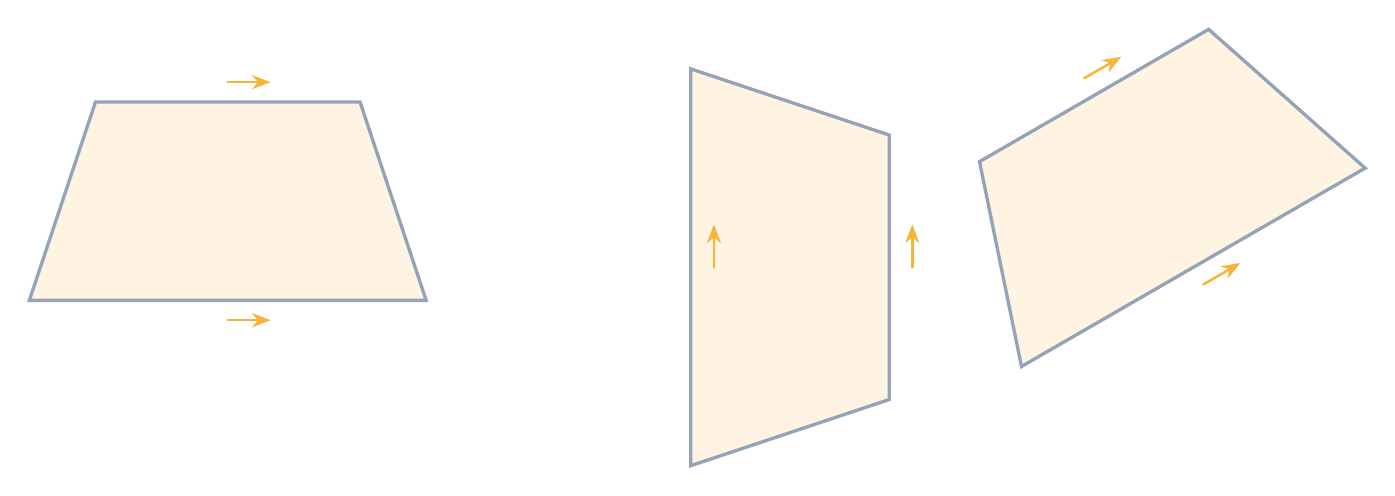
\begin{tikzpicture}[x=0.42cm,y=0.42cm,line cap=round,
  every node/.style={text=teks,font=\small}]
  \def\trap{ (0,0) -- (12,0) -- (10,6) -- (2,6) -- cycle }

  % 1: berdiri
  \begin{scope}[shift={(0,0)}]
    \fill[aksen!15] \trap;
    \draw[very thick,garis] \trap;
    \draw[-{Stealth[length=2.4mm]},aksen,line width=0.9pt]
      ($(0,0)!0.5!(12,0)+(0,-0.6)$) -- ($(0,0)!0.5!(12,0)+(1.3,-0.6)$);
    \draw[-{Stealth[length=2.4mm]},aksen,line width=0.9pt]
      ($(2,6)!0.5!(10,6)+(0,0.6)$) -- ($(2,6)!0.5!(10,6)+(1.3,0.6)$);
  \end{scope}

  % 2: diputar -90
  \begin{scope}[shift={(20,7)},rotate=-90]
    \fill[aksen!15] \trap;
    \draw[very thick,garis] \trap;
    \draw[-{Stealth[length=2.4mm]},aksen,line width=0.9pt]
      ($(0,0)!0.5!(12,0)+(0,0.7)$) -- ($(0,0)!0.5!(12,0)+(-1.3,0.7)$);
    \draw[-{Stealth[length=2.4mm]},aksen,line width=0.9pt]
      ($(2,6)!0.5!(10,6)+(0,0.7)$) -- ($(2,6)!0.5!(10,6)+(-1.3,0.7)$);
  \end{scope}

  % 3: miring 30 derajat
  \begin{scope}[shift={(30,-2)},rotate=30]
    \fill[aksen!15] \trap;
    \draw[very thick,garis] \trap;
    \draw[-{Stealth[length=2.4mm]},aksen,line width=0.9pt]
      ($(0,0)!0.5!(12,0)+(0,-0.6)$) -- ($(0,0)!0.5!(12,0)+(1.3,-0.6)$);
    \draw[-{Stealth[length=2.4mm]},aksen,line width=0.9pt]
      ($(2,6)!0.5!(10,6)+(0,0.6)$) -- ($(2,6)!0.5!(10,6)+(1.3,0.6)$);
  \end{scope}
\end{tikzpicture}
\end{document}
